\documentclass[11pt,a4paper]{article}

\usepackage[margin=2.4cm]{geometry}
\usepackage[utf8]{inputenc}
\usepackage[T1]{fontenc}
\usepackage{xcolor}
\usepackage{graphicx}
\usepackage{booktabs}
\usepackage{longtable}
\usepackage{array}
\usepackage{enumitem}
\usepackage{tikz}
\usetikzlibrary{arrows.meta,positioning,fit,backgrounds,shapes.geometric}
\usepackage{hyperref}
\usepackage{fancyhdr}
\usepackage{titlesec}
\setlength{\parindent}{0pt}
\setlength{\parskip}{0.6em}

\definecolor{inkdark}{HTML}{14181F}
\definecolor{accent}{HTML}{2D5A8C}
\definecolor{accentlight}{HTML}{7DB4E8}
\definecolor{muted}{HTML}{5A6472}
\definecolor{pass}{HTML}{3A8F5C}
\definecolor{warn}{HTML}{B8923A}
\definecolor{fail}{HTML}{B8383F}
\definecolor{panelbg}{HTML}{F5F6F8}
\definecolor{panelborder}{HTML}{D8DCE2}

\hypersetup{
  colorlinks=true,
  linkcolor=accent,
  urlcolor=accent,
  citecolor=accent,
  pdftitle={Email Header Analyzer with Threat Intelligence},
  pdfauthor={M. Ismail},
  pdfsubject={Technical Whitepaper}
}

\titleformat{\section}{\normalfont\Large\bfseries\color{inkdark}}{\thesection}{0.6em}{}
\titleformat{\subsection}{\normalfont\large\bfseries\color{inkdark}}{\thesubsection}{0.6em}{}
\titlespacing*{\section}{0pt}{1.6em}{0.8em}

\pagestyle{fancy}
\fancyhf{}
\renewcommand{\headrulewidth}{0.4pt}
\fancyhead[L]{\small\color{muted}Email Header Analyzer — Technical Whitepaper}
\fancyhead[R]{\small\color{muted}\thepage}

\newcommand{\note}[1]{\par\noindent\colorbox{panelbg}{\parbox{\dimexpr\linewidth-2\fboxsep}{\small #1}}\par\vspace{0.4em}}

\begin{document}

% ---------------------------------------------------------------------------
\begin{titlepage}
\centering
\vspace*{3cm}
{\Huge\bfseries Email Header Analyzer\par}
\vspace{0.4cm}
{\Large with Independent Verification and Threat Intelligence\par}
\vspace{1.6cm}
{\large A tool that turns a raw email header into an evidence-backed, explainable verdict\par}
\vspace{2.5cm}
{\large M. Ismail \par}
{\large SOC Internee, Ebryx \par}
\vspace{0.4cm}
{\normalsize Reviewer: Syed Jawad\par}
\vspace{2cm}
{\normalsize Technical Whitepaper \par}
{\normalsize \today \par}
\vfill
{\small MIT Licensed \textbullet\ repository link to be added on publish \par}
\end{titlepage}

\tableofcontents
\newpage

% ---------------------------------------------------------------------------
\section{Abstract}

Email header analysis is a core SOC triage skill, but most open tooling stops at
\emph{parsing}: it displays what a header says without checking whether any of it is true.
This project takes a raw email header, reconstructs the delivery path, \textbf{independently
re-evaluates} SPF, DKIM and DMARC against live DNS rather than trusting what the receiving
server recorded, extracts indicators of compromise, enriches them against real threat-intelligence
APIs, and produces a verdict where every contributing claim is traceable to a specific header
line. The design goal, stated plainly in the project's own planning document: \emph{every claim
the tool makes on screen must be one the analyst can justify from the evidence shown next to it}.
No opaque scores, no fabricated intelligence, no verdict without its reasons.

This document describes the architecture, the independent-verification approach that
differentiates it from parse-only tools, the risk-scoring model, the threat-intelligence
integration, and the engineering decisions behind each — including the deliberate
deviations from the original build brief and why each was made.

% ---------------------------------------------------------------------------
\section{Problem Statement}

A SOC analyst receiving a reported phishing email is handed a raw header and asked: is this
real? The manual answer requires several independent checks — read the \texttt{Received:}
chain bottom-up, compare \texttt{From}/\texttt{Reply-To}/\texttt{Return-Path} organisations,
re-derive SPF and DKIM against current DNS (because a header's recorded
\texttt{Authentication-Results} can simply be forged — RFC~8601 \S7.1 says so explicitly),
check DMARC alignment and policy, and cross-reference any IPs, domains or URLs against
threat intelligence. Existing open tools reviewed for this project (see
Section~\ref{sec:reference}) automate the parsing step but not the verification step: they
display whatever the header claims, including claims an attacker fully controls.

The tool built here automates the full manual workflow — not just the parsing half of it —
so its output is something an analyst can put directly into a ticket, with the reasoning
attached.

% ---------------------------------------------------------------------------
\section{Architecture Overview}

The application is a server-rendered FastAPI service. There is deliberately no database, no
queue and no cache server — analysis is synchronous, reports live in a bounded in-memory TTL
cache, and nothing outlives the process. This is a considered choice, not an omission: a
reference project reviewed during planning shipped PostgreSQL, Redis and Celery and used
none of them meaningfully (Section~\ref{sec:reference}).

\begin{figure}[h]
\centering
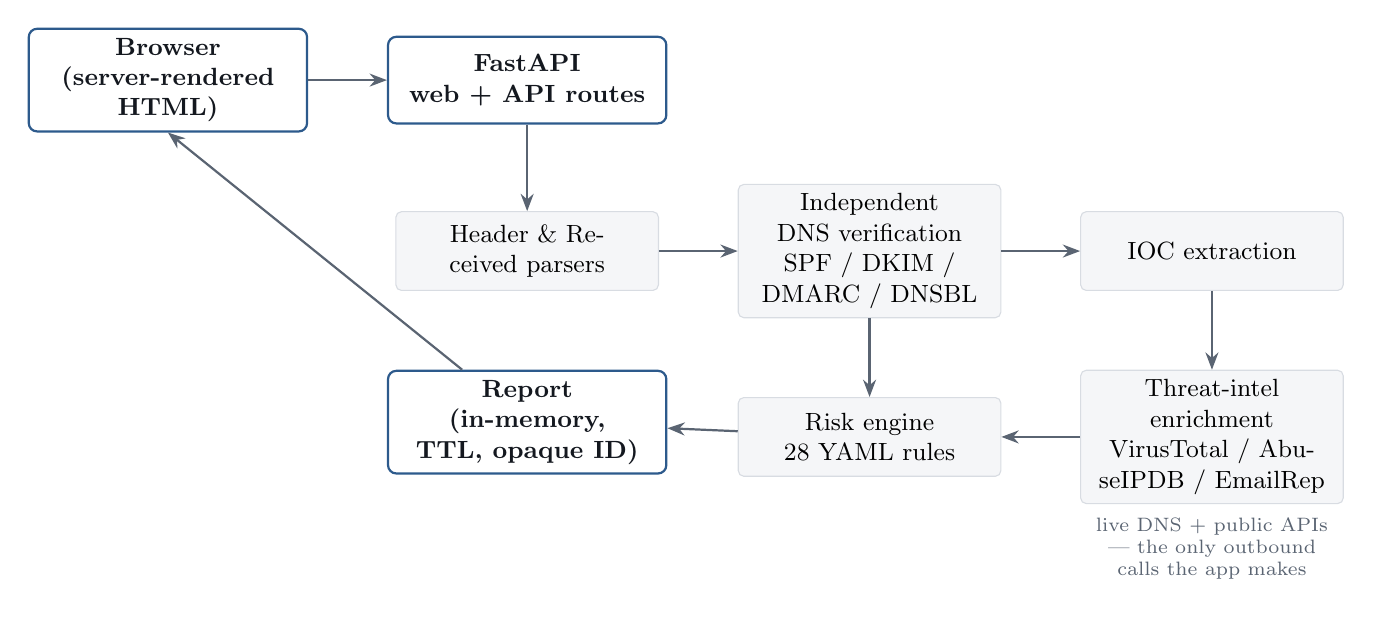
\begin{tikzpicture}[
  box/.style={draw=panelborder, fill=panelbg, rounded corners=2pt, minimum height=1cm, text width=3.1cm, align=center, font=\small},
  bigbox/.style={draw=accent, thick, rounded corners=3pt, minimum height=1.1cm, text width=3.3cm, align=center, font=\small\bfseries, text=inkdark},
  arr/.style={-{Stealth[length=2.2mm]}, thick, color=muted},
  node distance=0.9cm and 1.0cm
]
  \node[bigbox] (browser) {Browser\\(server-rendered HTML)};
  \node[bigbox, right=of browser] (fastapi) {FastAPI\\web + API routes};
  \node[box, below=1.1cm of fastapi] (parse) {Header \& Received parsers};
  \node[box, right=of parse] (verify) {Independent DNS verification\\SPF / DKIM / DMARC / DNSBL};
  \node[box, right=of verify] (ioc) {IOC extraction};
  \node[box, below=1.0cm of ioc] (enrich) {Threat-intel enrichment\\VirusTotal / AbuseIPDB / EmailRep};
  \node[box, below=1.0cm of verify] (risk) {Risk engine\\28 YAML rules};
  \node[bigbox, below=1.0cm of parse] (report) {Report\\(in-memory, TTL, opaque ID)};

  \draw[arr] (browser) -- (fastapi);
  \draw[arr] (fastapi) -- (parse);
  \draw[arr] (parse) -- (verify);
  \draw[arr] (verify) -- (ioc);
  \draw[arr] (ioc) -- (enrich);
  \draw[arr] (verify) -- (risk);
  \draw[arr] (enrich) -- (risk);
  \draw[arr] (risk) -- (report);
  \draw[arr] (report) -- (browser.south) [bend right=18];

  \node[font=\scriptsize, color=muted, below=0.05cm of enrich, text width=3.3cm, align=center] {live DNS + public APIs — the only outbound calls the app makes};
\end{tikzpicture}
\caption{Request lifecycle. Live outbound network calls happen in exactly two places:
DNS resolution during verification, and threat-intel HTTP calls during enrichment
(opt-in, off by default).}
\end{figure}

\subsection{Module boundaries}
\begin{itemize}[leftmargin=1.4em]
  \item \textbf{\texttt{app/core/}} — pure analysis logic: header parsing, \texttt{Received:}
    chain reconstruction, authentication parsing, identity comparison, IOC extraction, domain
    analysis (lookalike/homoglyph detection), the risk engine. No I/O.
  \item \textbf{\texttt{app/core/verification/}} — independent SPF/DKIM/DMARC/DNSBL/FCrDNS
    evaluation. The only place live DNS is queried.
  \item \textbf{\texttt{app/integrations/}} — one file per threat-intel provider, each behind
    a common \texttt{Provider} interface.
  \item \textbf{\texttt{app/services/}} — orchestration: \texttt{analysis\_service} ties
    parsing, verification, enrichment and risk scoring into one report;
    \texttt{enrichment\_service} owns concurrency limits, caching and demo-mode fixtures;
    \texttt{report\_service} owns JSON/Markdown/PDF export.
  \item \textbf{\texttt{app/routes/}} — HTTP surface: server-rendered pages (\texttt{web.py}),
    a typed JSON API (\texttt{api.py}), report export endpoints.
\end{itemize}

% ---------------------------------------------------------------------------
\section{Parsing Pipeline}

\begin{figure}[h]
\centering
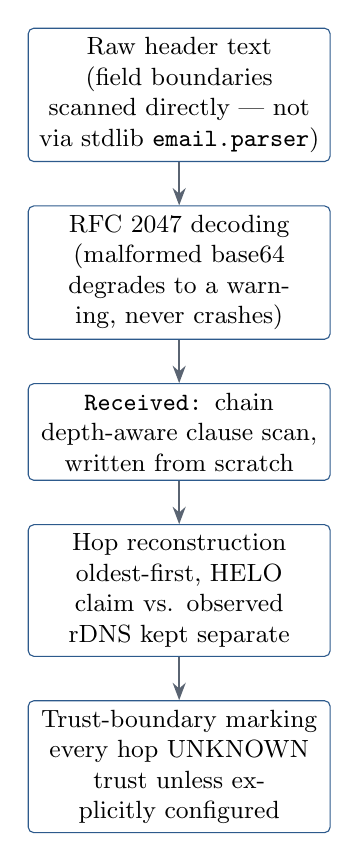
\begin{tikzpicture}[
  pstep/.style={draw=accent, fill=white, rounded corners=2pt, minimum height=0.9cm, text width=3.6cm, align=center, font=\small},
  arr/.style={-{Stealth[length=2.2mm]}, thick, color=muted},
  node distance=0.55cm
]
  \node[pstep] (a) {Raw header text\\(field boundaries scanned directly — not via stdlib \texttt{email.parser})};
  \node[pstep, below=of a] (b) {RFC 2047 decoding\\(malformed base64 degrades to a warning, never crashes)};
  \node[pstep, below=of b] (c) {\texttt{Received:} chain\\depth-aware clause scan, written from scratch};
  \node[pstep, below=of c] (d) {Hop reconstruction\\oldest-first, HELO claim vs. observed rDNS kept separate};
  \node[pstep, below=of d] (e) {Trust-boundary marking\\every hop UNKNOWN trust unless explicitly configured};
  \draw[arr] (a) -- (b);
  \draw[arr] (b) -- (c);
  \draw[arr] (c) -- (d);
  \draw[arr] (d) -- (e);
\end{tikzpicture}
\caption{Header parsing preserves raw bytes, original field order and duplicate headers —
information a stdlib-\texttt{email}-based parser silently discards.}
\end{figure}

The \texttt{Received:} parser is written from scratch. The best available open
\texttt{Received:} parser (\texttt{eml\_parser}, GOVCERT-LU) was evaluated and rejected: it is
AGPL-3.0, and \S13 of that licence triggers on any network-served use of the work — exactly
what this application is. Reimplementing it clean-room was the only option compatible with an
MIT-licensed, publishable project.

% ---------------------------------------------------------------------------
\section{Independent Verification}
\label{sec:verification}

This is the project's primary differentiator. Every one of the six reference open-source
tools audited during planning (Section~\ref{sec:reference}) is parse-only: they read whatever
\texttt{Authentication-Results} the receiving server wrote and display it as-is. RFC~8601
\S7.1 is explicit that this header is forgeable — an attacker can place
\texttt{Authentication-Results: yourcompany.com; spf=pass; dkim=pass; dmarc=pass} into a
message they compose themselves, and a tool that reads it uncritically shows a green pass.

\begin{figure}[h]
\centering
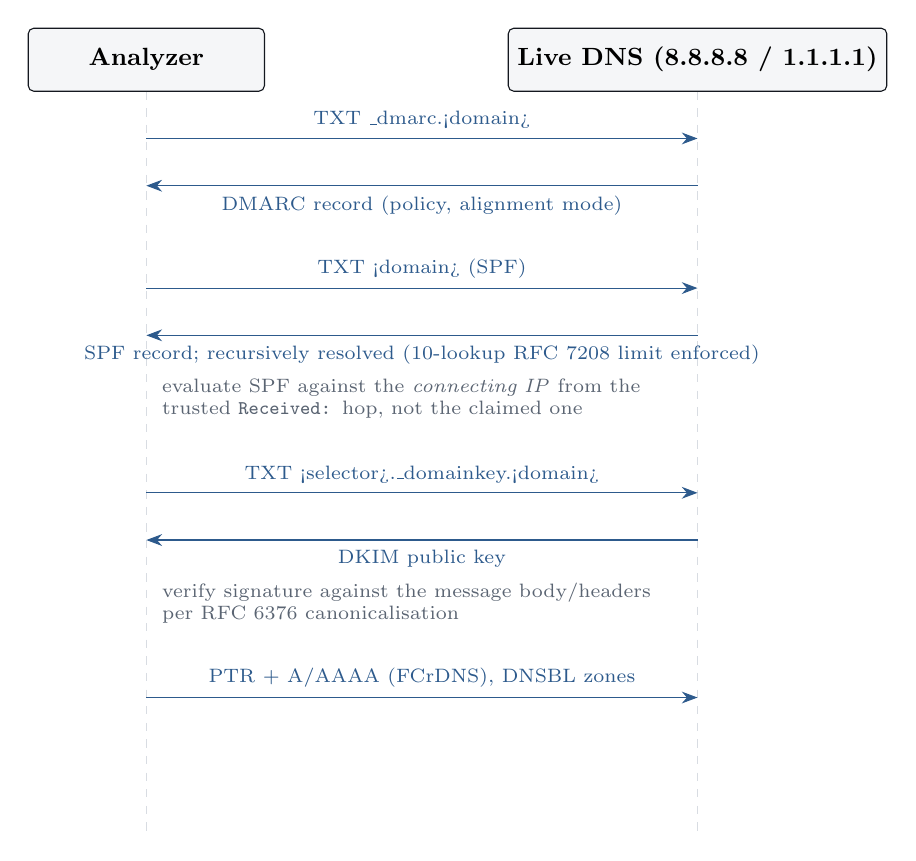
\begin{tikzpicture}[
  actor/.style={draw=inkdark, fill=panelbg, rounded corners=2pt, minimum height=0.8cm, minimum width=3cm, align=center, font=\small\bfseries},
  msg/.style={-{Stealth[length=2mm]}, color=accent},
  lifeline/.style={draw=panelborder, dashed}
]
  \node[actor] (analyzer) at (0,0) {Analyzer};
  \node[actor] (dns) at (7,0) {Live DNS (8.8.8.8 / 1.1.1.1)};
  \draw[lifeline] (analyzer.south) -- ++(0,-9.4);
  \draw[lifeline] (dns.south) -- ++(0,-9.4);

  \draw[msg] (0,-1.0) -- node[above,font=\scriptsize]{TXT \_dmarc.<domain>} (7,-1.0);
  \draw[msg] (7,-1.6) -- node[below,font=\scriptsize]{DMARC record (policy, alignment mode)} (0,-1.6);

  \draw[msg] (0,-2.9) -- node[above,font=\scriptsize]{TXT <domain> (SPF)} (7,-2.9);
  \draw[msg] (7,-3.5) -- node[below,font=\scriptsize]{SPF record; recursively resolved (10-lookup RFC 7208 limit enforced)} (0,-3.5);

  \node[font=\scriptsize, align=left, text width=6.6cm, color=muted] at (3.5,-4.3) {evaluate SPF against the \emph{connecting IP} from the trusted \texttt{Received:} hop, not the claimed one};

  \draw[msg] (0,-5.5) -- node[above,font=\scriptsize]{TXT <selector>.\_domainkey.<domain>} (7,-5.5);
  \draw[msg] (7,-6.1) -- node[below,font=\scriptsize]{DKIM public key} (0,-6.1);

  \node[font=\scriptsize, align=left, text width=6.6cm, color=muted] at (3.5,-6.9) {verify signature against the message body/headers per RFC 6376 canonicalisation};

  \draw[msg] (0,-8.1) -- node[above,font=\scriptsize]{PTR + A/AAAA (FCrDNS), DNSBL zones} (7,-8.1);
\end{tikzpicture}
\caption{Independent verification queries live DNS itself rather than trusting the recorded
\texttt{Authentication-Results:} header. Results are shown \emph{asserted vs.\ verified},
side by side, on the results page.}
\end{figure}

\subsection{What "asserted" vs. "verified" means on screen}

Every authentication row in the results UI shows both what was \emph{asserted} (what the
receiving infrastructure claimed, with a trust level — \texttt{UNKNOWN} unless the deployment
explicitly configures \texttt{TRUSTED\_RECEIVER\_DOMAINS}) and what was \emph{independently
verified} (what this tool itself derived from live DNS, right now). The two can disagree —
that disagreement is itself surfaced as evidence, not hidden.

\subsection{Correctness bugs this differentiator actually caught}
Three real defects were found by the project's own test suite while building this layer, each
worth stating because they show why "verify it yourself" is harder than it sounds:
\begin{enumerate}[leftmargin=1.4em]
  \item \texttt{email.header.decode\_header} raises \texttt{HeaderParseError}, which is
    \emph{not} a \texttt{ValueError} subclass — a malformed base64 encoded-word escaped the
    exception handler entirely before this was caught and degraded to a warning.
  \item \texttt{.example} is not in the Public Suffix List. \texttt{tldextract} returned no
    suffix for it, so \texttt{mail.bank.example} and \texttt{bank.example} compared as
    \emph{unrelated} organisations — silently defeating the impersonation check on every
    test fixture. Fixed with a documented last-two-labels fallback.
  \item \texttt{pyspf} dispatches DNS through a module-level resolver and treats an empty
    cache entry as a cache miss. Seeding its cache for offline tests did not actually prevent
    it — the test suite was silently performing live DNS lookups. In production this meant
    every \texttt{include:}/\texttt{a:}/\texttt{redirect=} directive bypassed the configured
    resolver and timeout entirely. Fixed by patching the resolver dispatch point directly.
\end{enumerate}

% ---------------------------------------------------------------------------
\section{Indicators of Compromise and Threat-Intelligence Enrichment}

\begin{figure}[h]
\centering
\resizebox{\linewidth}{!}{%
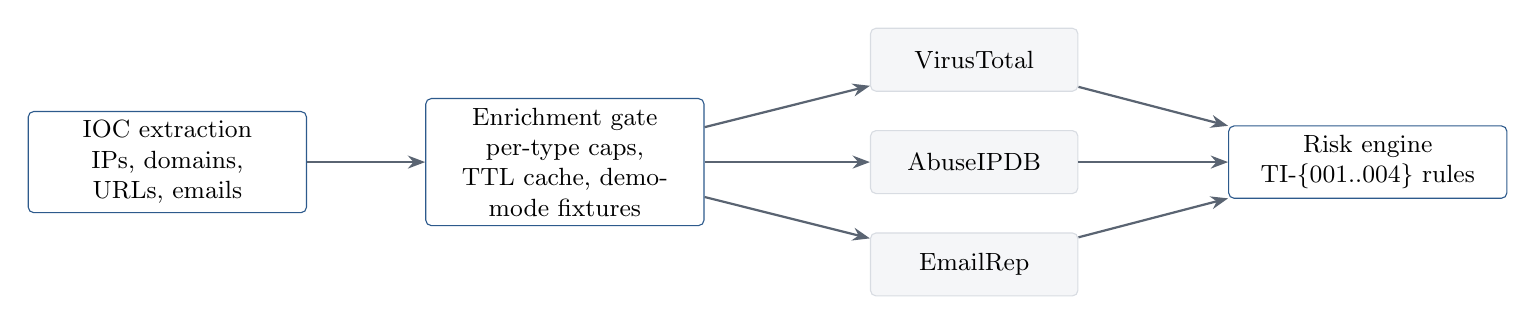
\begin{tikzpicture}[
  pstep/.style={draw=accent, fill=white, rounded corners=2pt, minimum height=0.85cm, text width=3.3cm, align=center, font=\small},
  prov/.style={draw=panelborder, fill=panelbg, rounded corners=2pt, minimum height=0.8cm, minimum width=2.4cm, text width=2.4cm, align=center, font=\small},
  arr/.style={-{Stealth[length=2.2mm]}, thick, color=muted},
]
  \node[pstep] (extract) at (0,0) {IOC extraction\\IPs, domains, URLs, emails};
  \node[pstep, right=1.5cm of extract] (gate) {Enrichment gate\\per-type caps, TTL cache, demo-mode fixtures};
  \node[prov, right=2.1cm of gate, yshift=1.3cm] (vt) {VirusTotal};
  \node[prov, right=2.1cm of gate] (abuse) {AbuseIPDB};
  \node[prov, right=2.1cm of gate, yshift=-1.3cm] (rep) {EmailRep};
  \node[pstep, right=1.9cm of abuse] (risk) {Risk engine\\TI-\{001..004\} rules};

  \draw[arr] (extract) -- (gate);
  \draw[arr] (gate) -- (vt);
  \draw[arr] (gate) -- (abuse);
  \draw[arr] (gate) -- (rep);
  \draw[arr] (vt) -- (risk);
  \draw[arr] (abuse) -- (risk);
  \draw[arr] (rep) -- (risk);
\end{tikzpicture}%
}
\caption{Enrichment is a single deliberate gate (\texttt{enrichment\_service.py}): it, and
nothing else, decides whether a provider is ever called. Providers themselves never know
about caching, per-type limits or demo mode.}
\end{figure}

\subsection{Off by default, on purpose}
\texttt{ENRICHMENT\_ENABLED} defaults to \texttt{false}. This is deliberate, not a missing
feature: enabling it sends extracted indicators to third parties, and phishing URLs are
frequently unique per recipient — submitting one to a public scanner can itself signal to the
attacker that their campaign was detected. Turning enrichment on is an explicit operator
decision, never an inherited default.

\subsection{Providers}
\begin{itemize}[leftmargin=1.4em]
  \item \textbf{VirusTotal} — IPs, domains and URLs, checked against up to 90+ vendor engines.
  \item \textbf{AbuseIPDB} — IP abuse-report history and confidence score. Country code is
    captured for display only; it is asserted by test
    (\texttt{test\_country\_never\_contributes\_to\_score}) that it never influences the risk
    score.
  \item \textbf{EmailRep} — sender-address reputation, feeding directly into the "why this
    verdict" evidence for BEC/impersonation findings.
\end{itemize}

Every lookup — including a \texttt{DISABLED} one — is recorded and shown. The UI never
silently omits a check that wasn't run; it says so explicitly, because "not checked" and
"checked and clean" are different findings and conflating them is a false sense of safety.

\subsection{Verified against live providers}
The threat-intelligence path in Figure 4 was exercised end-to-end against the real APIs (not
mocked) as part of this project's own verification: Figure~\ref{fig:threat-intel-live} shows
the actual response.

\begin{figure}[h]
\centering
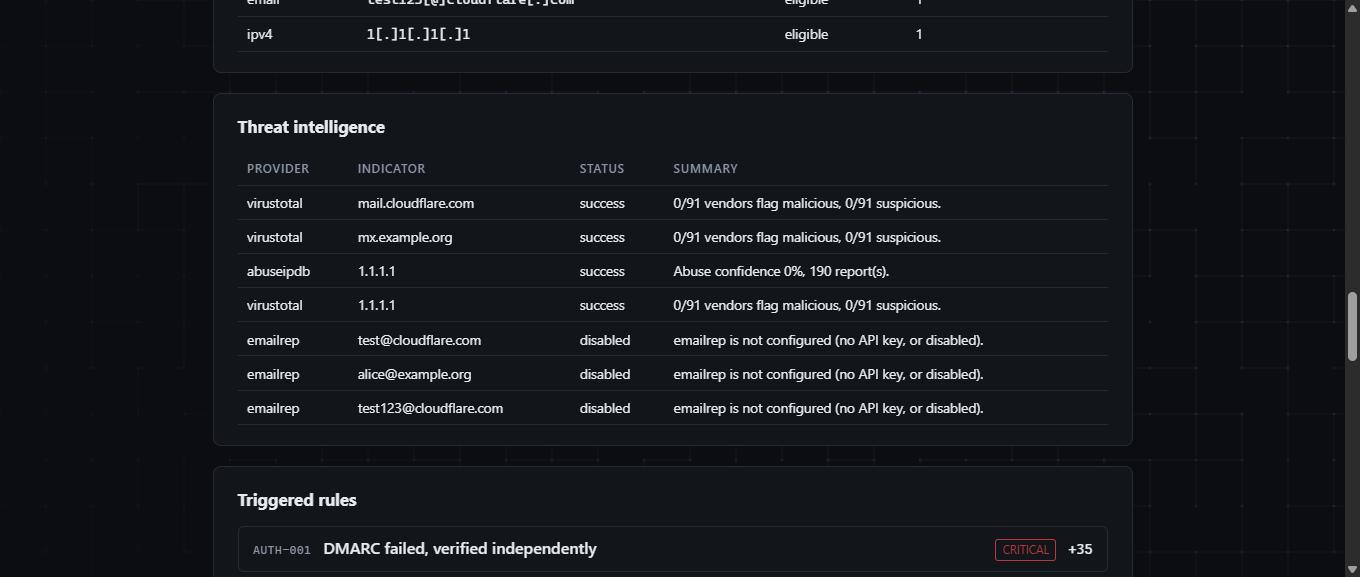
\includegraphics[width=\linewidth]{figures/threat-intel-live.jpg}
\caption{Live enrichment results for a test message — real VirusTotal and AbuseIPDB API
responses, not fixtures. \texttt{1.1.1.1} returns 0/91 vendors flagging malicious from
VirusTotal and 0\% abuse confidence with 190 historical reports from AbuseIPDB. EmailRep
shows \texttt{disabled} here because no API key was configured for that provider at
capture time — exactly the "not checked, not clean" distinction described above.}
\label{fig:threat-intel-live}
\end{figure}

% ---------------------------------------------------------------------------
\section{Risk Engine and Verdict}

Risk rules are declared in YAML (\texttt{app/core/rules/rules.yaml}), not embedded in Python —
28 rules at time of writing, each with a stable ID (e.g. \texttt{AUTH-001},
\texttt{IDN-002}, \texttt{RTE-004}, \texttt{TI-004}), an evidence strength, a score
contribution, and, critically, a \emph{possible legitimate explanation} and a
\emph{recommended action}. This lets the verdict card name exactly which rules fired, in
plain language, reviewable by someone who has never read the Python.

\subsection{Correlate, don't override}
The engine deliberately has no single rule that can unilaterally declare a verdict. Evidence
accumulates; the final verdict is a function of the accumulated score and the confidence in
that score, not any one rule short-circuiting the rest. The exception is explicit and visible:
if a \emph{matched pattern} (a named, high-confidence combination) fires, it is surfaced as
\texttt{risk.matched\_pattern} on the verdict — but it still contributes through the same
scoring path, not as a bypass.

\subsection{What the verdict deliberately cannot say}
There is no \texttt{SAFE} verdict and no \texttt{BEC\_CONFIRMED} verdict. Header evidence
cannot establish that a message is harmless — a compromised but genuine mailbox passes every
authentication check there is — and it cannot establish business context, which an actual BEC
determination requires. The five possible verdicts are \emph{Likely Legitimate (based on
available header evidence)}, \emph{Suspicious}, \emph{Likely Phishing}, \emph{Possible
BEC/Impersonation}, and \emph{Inconclusive}. Every one of them is a statement about the
evidence, not a claim about ground truth.

% ---------------------------------------------------------------------------
\section{Evidence-Backed Verdict: Worked Example}

Figure~\ref{fig:verdict-phishing} shows the bundled phishing sample run through the tool with
live threat-intel enrichment on. The verdict card states a score and a confidence level;
immediately below it, the \emph{Why this verdict} panel lists the specific evidence, each
citation naming the exact header field and value that produced it — not a generic "this looks
suspicious," but "Reply-To is \texttt{support@secure-verify-alerts.example}, but From is in
\texttt{northw1nd-secure.example}. Replies leave the sender's organisation," with a link to
the raw header line it was read from.

\begin{figure}[h]
\centering
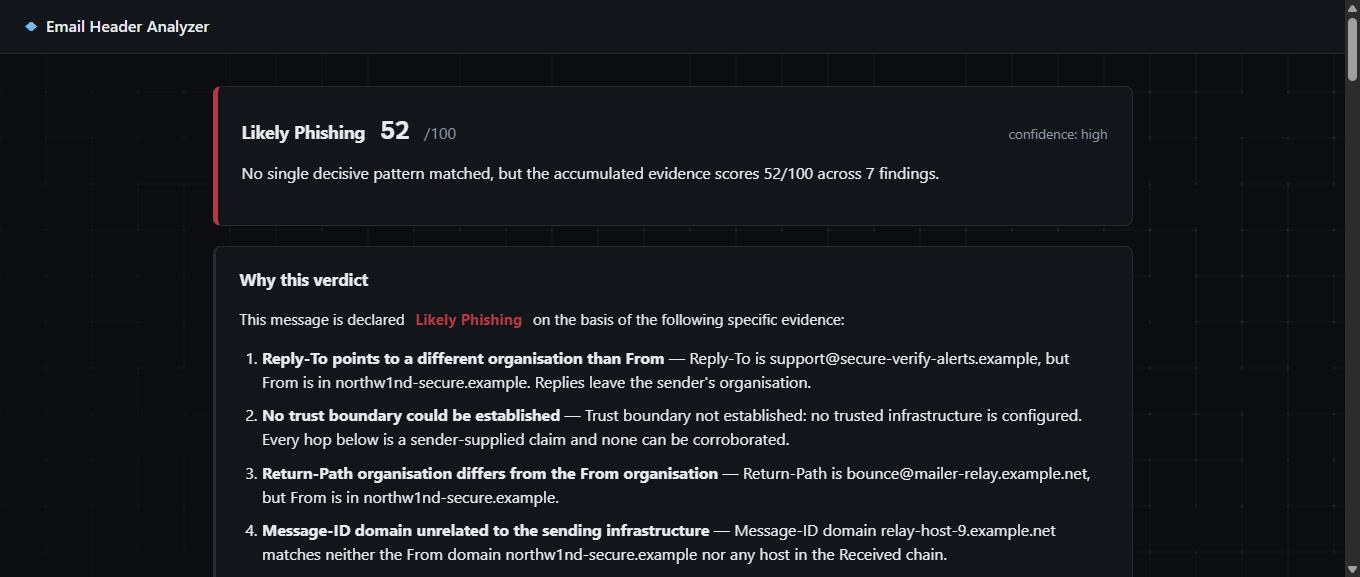
\includegraphics[width=\linewidth]{figures/verdict-phishing.jpg}
\caption{Evidence-backed verdict for the bundled phishing sample. Every numbered citation
traces to a specific header field; the full findings list below it (not shown) adds, for each
finding, why it matters, a possible legitimate explanation, and a recommended action.}
\label{fig:verdict-phishing}
\end{figure}

% ---------------------------------------------------------------------------
\section{Interface}

Server-rendered Jinja2 templates, not a client-side framework — a deliberate deviation from
the original brief's Bootstrap/React-leaning suggestion. Two reasons: Jinja2 autoescaping is
the primary XSS defence against input that is, by definition, attacker-controlled (a raw email
header); and a server-rendered app with no build step and no CDN dependency works air-gapped,
which several reference tools do not.

\begin{figure}[h]
\centering
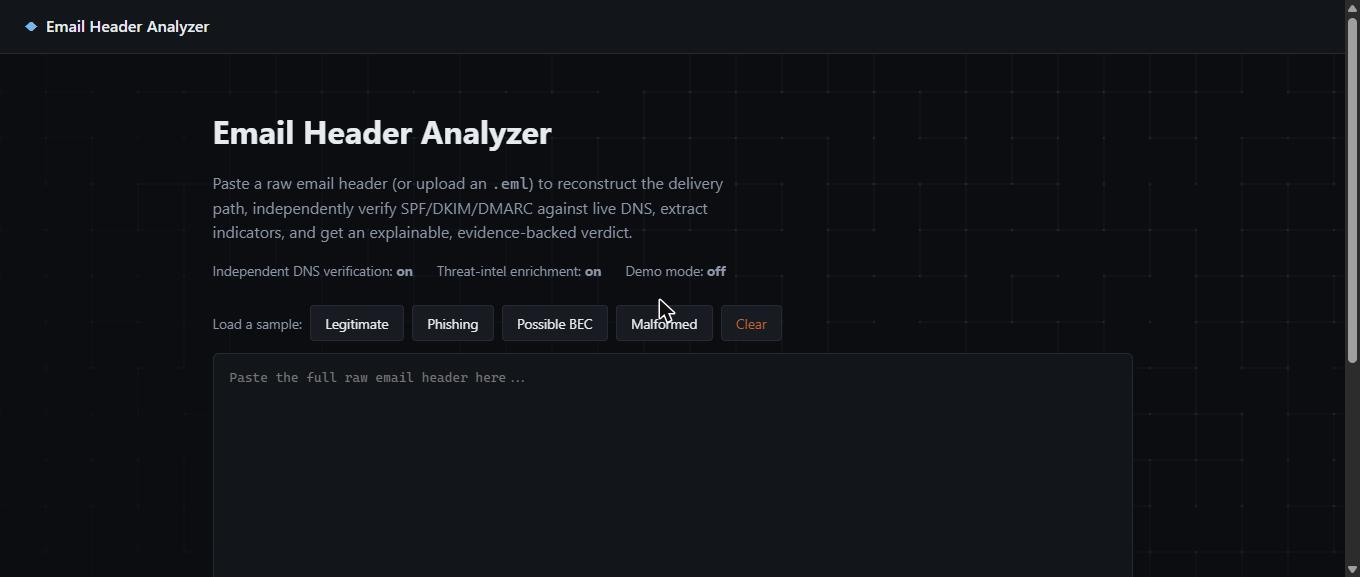
\includegraphics[width=0.92\linewidth]{figures/landing.jpg}
\caption{Landing page. Configuration state (DNS verification, threat-intel enrichment, demo
mode) is always visible, never implicit — an analyst should never have to guess what a given
run actually checked.}
\end{figure}

\begin{figure}[h]
\centering
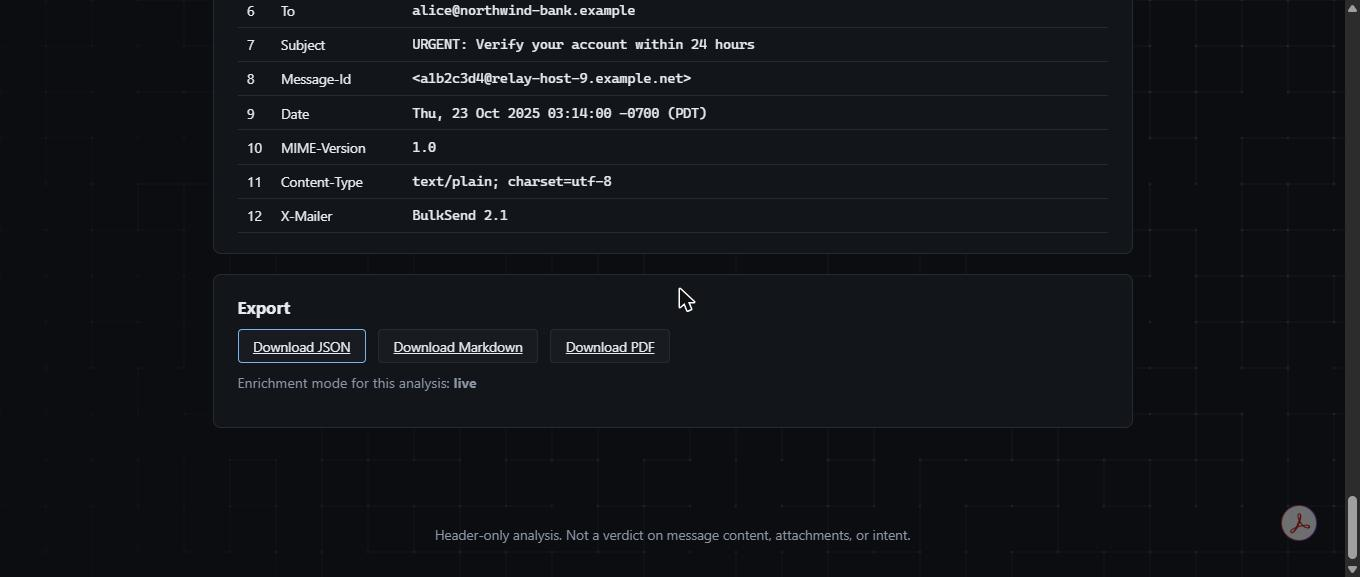
\includegraphics[width=0.92\linewidth]{figures/export-panel.jpg}
\caption{Export panel. Reports export as JSON (for tooling), Markdown (for a ticket or wiki
page), or PDF — a standalone, print-formatted document generated server-side via a
pure-Python HTML-to-PDF pipeline (\texttt{xhtml2pdf}), chosen specifically because it needs
no external binary (no headless Chrome, no \texttt{wkhtmltopdf}, no GTK), so it installs
cleanly cross-platform including Windows.}
\end{figure}

% ---------------------------------------------------------------------------
\section{Design Decisions and Deviations from the Brief}

The original build brief was used as a requirements baseline; the table below records where
this implementation deviates from it and why, each decision made after auditing prior art
rather than by default.

\renewcommand{\arraystretch}{1.25}
\begin{longtable}{@{}p{0.9cm}p{5.6cm}p{9.4cm}@{}}
\toprule
\textbf{ID} & \textbf{Decision} & \textbf{Rationale} \\
\midrule
\endhead
ADR-01 & Kept the real-customer-data case study out of this repository & The Ebryx case
report used to develop the manual methodology contains real customer headers and employee
addresses; this repository is intended to be published, so it lives entirely separately. \\
ADR-02 & Clean-room implementation, no third-party code reused & Four of eight reference
projects audited grant no reuse rights at all; two more are GPL-3.0 despite GitHub or their
own README misreporting the licence. \\
ADR-03 & Implements live DNS/cryptographic verification & The differentiator; every reference
project audited is parse-only. \\
ADR-04 & No database, queue or cache server & Nothing needs to persist; avoids the
dead-infrastructure failure mode observed in a reference project (PostgreSQL + Redis + Celery,
none used meaningfully). \\
ADR-05 & Offline by default, enrichment strictly opt-in & Analysts are frequently forbidden
from submitting customer indicators to third parties; unique-per-recipient phishing URLs can
tip off an attacker if submitted to a public scanner. \\
ADR-06 & Server-rendered Jinja2, no client framework & Autoescaping is the primary XSS defence
on hostile input; no build step, no CDN dependency. \\
ADR-07 & Risk rules externalised to YAML with stable IDs & Lets the verdict cite exactly which
rules fired, reviewable without reading Python. \\
ADR-08 & \texttt{tldextract} with network fetch disabled, bundled PSL snapshot & A security
tool making an unannounced outbound HTTP request during analysis is itself a finding. \\
\bottomrule
\end{longtable}

% ---------------------------------------------------------------------------
\section{Threat Model and Limitations}

\subsection{What this tool is not}
This is header-only analysis. It makes no claim about message body content, attachments, or
sender intent — the footer on every results page says so explicitly. It cannot establish that
a message is safe: a compromised-but-genuine account passes every check here. Independent
verification checks \emph{current} DNS state, which can differ from what was published at
delivery time (a domain can rotate SPF/DKIM records after the fact).

\subsection{Trust boundary}
\texttt{Authentication-Results} headers are forgeable per RFC~8601 \S7.1. Every asserted
result defaults to \texttt{UNKNOWN} trust unless \texttt{TRUSTED\_RECEIVER\_DOMAINS} /
\texttt{TRUSTED\_RECEIVER\_HOSTS} is explicitly configured to name infrastructure the operator
actually controls. Leaving this unset is the safe default, not a bug.

\subsection{Data handling}
Raw headers are never placed in a URL or query parameter (asserted structurally by test —
every route accepting header content is a POST-body route, checked by walking the FastAPI
route table itself). \texttt{LOG\_RAW\_HEADERS} defaults to \texttt{false}. Reports live in a
bounded, short-lived, in-memory cache with opaque IDs (\texttt{secrets.token\_urlsafe}), never
derived from message content.

% ---------------------------------------------------------------------------
\section{Testing and Quality}

253 tests pass with no network access and no API keys required for the suite itself (the live
threat-intel path is exercised separately and manually, as in Figure~\ref{fig:threat-intel-live},
never as part of CI). The suite includes architectural boundary tests — e.g. asserting the
core analysis modules perform no I/O — and structural security tests, such as walking
FastAPI's route table to assert no GET route can expose header content via a path parameter.
Linting is enforced with \texttt{ruff}; every rule suppression in \texttt{pyproject.toml} is
documented with a one-line rationale rather than left silent.

A test-isolation gap was found and fixed during this documentation pass: \texttt{Settings}
reads \texttt{.env} from the working directory by pydantic-settings default, so a developer's
local \texttt{.env} — enrichment keys, feature flags — silently leaked into any test that
built a bare \texttt{Settings()} without explicitly overriding every affected field. Fixed with
a session-scoped \texttt{conftest.py} fixture that disables the dotenv source for the whole
test session, so test behaviour no longer depends on what happens to be sitting in the repo
root.

% ---------------------------------------------------------------------------
\section{Reference Repositories}
\label{sec:reference}

Eight open-source projects were audited before implementation began, for licence terms and
reusable concepts. Two licence traps were found and are worth recording: one project is
reported as "Other" by GitHub's licence detector when it is actually GPL-3.0; another's README
claims MIT while its actual \texttt{LICENSE} file is GPL-3.0. Four of the eight grant no reuse
rights at all. The conclusion drawn — clean-room implementation throughout, no third-party
code — is ADR-02 above. Full audit notes are in \texttt{docs/REFERENCE\_REPOSITORIES.md} in
the repository.

% ---------------------------------------------------------------------------
\section{Setup and Deployment}

\begin{itemize}[leftmargin=1.4em]
  \item \textbf{Local run:} \texttt{pip install -r requirements.txt}, copy \texttt{.env.example}
    to \texttt{.env}, \texttt{uvicorn app.main:app}. Works fully offline with zero
    configuration — every provider reports \texttt{DISABLED} rather than inventing a result.
  \item \textbf{Container:} a production Dockerfile and \texttt{docker-compose.yml} are
    provided.
  \item \textbf{Secrets:} \texttt{.env} is git-ignored; nothing in it is ever committed.
    \texttt{CSRF\_SECRET} should be generated per deployment
    (\texttt{python -c "import secrets; print(secrets.token\_urlsafe(32))"}).
\end{itemize}

% ---------------------------------------------------------------------------
\section{Conclusion}

The header-only, independently-verified, evidence-cited approach documented here is a direct
translation of a manual SOC workflow into software — not an approximation of one. Every design
decision recorded in Section~9 traces back either to a gap found in existing open tooling or to
a correctness bug the project's own test suite caught while building it. The result is a tool
whose verdict an analyst can defend under questioning, because the tool itself can point at the
exact line of evidence behind every claim it makes.

\end{document}
